\documentclass[12pt, twoside]{article}
\documentclass[12pt, twoside]{article}
\usepackage[letterpaper, margin=1in, headsep=0.2in]{geometry}
\setlength{\headheight}{0.6in}
%\usepackage[english]{babel}
\usepackage[utf8]{inputenc}
\usepackage{microtype}
\usepackage{amsmath}
\usepackage{amssymb}
%\usepackage{amsfonts}
\usepackage{siunitx} %units in math. eg 20\milli\meter
\usepackage{yhmath} % for arcs, overparenth command
\usepackage{tikz} %graphics
\usetikzlibrary{quotes, angles}
\usepackage{graphicx} %consider setting \graphicspath{{images/}}
\usepackage{parskip} %no paragraph indent
\usepackage{enumitem}
\usepackage{multicol}
\usepackage{venndiagram}

\usepackage{fancyhdr}
\pagestyle{fancy}
\fancyhf{}
\renewcommand{\headrulewidth}{0pt} % disable the underline of the header
\raggedbottom
\hfuzz=2mm %suppresses overfull box warnings

\usepackage{hyperref}
\usepackage{float}

\title{Algebra 2}
\author{Chris Huson}
\date{June 2024}

\fancyhead[LE]{\thepage}
\fancyhead[RO]{\thepage \\ Name: \hspace{1.5cm} \,\\}
\fancyhead[LO]{BECA/Huson/Algebra 2: Regents Preparation \\* 18 June 2024}

\begin{document}
\subsubsection*{Prep \#31 - Survey data}
\begin{enumerate}
\item Which statement about data collection is most accurate?
\begin{enumerate}
    \item A survey about parenting styles given to every tenth student entering the library will provide unbiased results.
    \item An observational study allows a researcher to determine the cause of an outcome.
    \item Margin of error increases as sample size increases.
    \item A survey collected from a random sample of students in a school can be used to represent the opinions of the school population.
\end{enumerate} %Regents Jan 2023

\item The Hot and Tasty Coffee chain conducts a survey of its customers at its location at the Staten Island ferry terminal. After the survey is completed, the statistical consultant states that 70\% of customers who took the survey said the most important factor in choosing where to get their coffee is how fast they are served. Based on this result, Hot and Tasty Coffee can infer that
\begin{enumerate}
    \item most of its customers in New York State care most about being served quickly
    \item coffee drinkers care less about taste and more about being served quickly
    \item most of its customers at the Staten Island ferry terminal care most about being served quickly
    \item most of its customers at transportation terminals and stations care most about being served quickly
\end{enumerate} %Regent Aug 2022

\item In watching auditions for lead singer in a band, Liem became curious as to whether there is an association between how animated the lead singer is and the amount of applause from the audience. He decided to watch each singer and rate the singer on a scale of 1 to 5, where 1 is the least animated and 5 is the most animated. He did this for all 5 nights of auditions and found that the more animated singers did receive louder applause. \\[0.25cm]
The study Liem conducted would be best described as %Regent Aug 2022
\begin{enumerate}
    \item experimental
    \item a sample survey
    \item observational
    \item a random assignment
\end{enumerate}


\newpage
\item Betty conducted a survey of her class to see if they like pizza. She gathered 200 responses and 65\% of the voters said they did like pizza. Betty then ran a simulation of 400 more surveys, each with 200 responses, assuming that 65\% of the voters would like pizza. The output of the simulation is shown below.
\begin{center}
    \begin{tikzpicture}[xscale=40, yscale=0.20]
        \draw[thick,-] (0.5,0) -- (0.8,0) node[below] {$x$};
        \draw[thick,-] (0.5,0) -- (0.5,15);
        \foreach \x in {0.55,0.60,0.65,0.70,0.75} {
            \draw (\x,0.1) -- (\x,-0.1) node[below] {\x};
        }
        \foreach \x/\value in {0.53/2,0.55/5,0.56/8,0.57/12,0.58/10,0.59/14,0.60/15,0.61/11,0.62/15,0.63/19,0.64/17,0.65/21,0.66/15,0.67/10,0.68/8,0.69/9,0.70/8,0.71/2,0.72/6,0.73/2,0.74/0,0.75/1} {
            \foreach \y in {0.5,1,...,\value} {
                \draw (\x,\y) node[circle, fill, inner sep=0.5pt] {};
            }
        }
        \node[rotate=90, font=\bfseries] at (0.48,7.5) {Frequency};
        \node[font=\bfseries] at (0.65,-4) {Proportion};
        \node at (0.75,12) {Mean = 0.654};
        \node at (0.75,10) {SD = 0.035};
    \end{tikzpicture}
    \end{center}
Considering the middle 95\% of the data, what is the margin of error for the simulation?
    \begin{multicols}{2}
        \begin{enumerate}
            \item 0.01
            \item 0.02
            \item 0.05
            \item 0.07
        \end{enumerate}
    \end{multicols} %Regents Jan 2023

\item State officials claim 82\% of a community want to repeal the 30 mph speed limit on an expressway. A community organization devises a simulation based on the claim that 82\% of the community supports the repeal. Each dot on the graph below represents the proportion of community members who support the repeal. The graph shows 200 simulated surveys, each of sample size 60.
\begin{center}
    \includegraphics*[width=7cm]{../graphics/norm-36-Aug2022.png}
\end{center}
Based on the simulation, determine an interval containing the middle 95\% of plausible proportions. Round your answer to the \emph{nearest thousandth}. \\[0.25cm]
The community organization conducted its own sample survey of 60 people and found 70\% supported the repeal. Based on the results of the simulation, explain why the organization should question the State officials' claim. \vspace{3cm} %Regent Aug 2022


\item A simulation of student response times is run and displayed as a histogram below.
    \begin{center}
    \begin{tikzpicture}[scale=0.55]
        \draw[thick,->] (0,0) -- (15.5,0) node[below] {$x$};
        \draw[thick,-] (0,0) -- (0,7.5);
        \foreach \x in {0,1,...,15} {
            \draw (\x,0.1) -- (\x,-0.1) node[below] {\x};
        }
        \foreach \x/\value in {1/1,2/4,3/5,4/7,5/10,6/11,7/12,8/9,9/9,10/7,11/3,12/2,13/3,14/1} {
            \foreach \y in {0.5,1,...,\value} {
                \fill (\x,\y+rand*0.005) circle (0.1);
            }
        }
    \end{tikzpicture}
    \end{center}
    \begin{enumerate}[itemsep=1.5cm]
        \item Estimate the mean response time, $\overline{x}$.
        \item Estimate the standard deviation of the response times, $\sigma$.
        \item Find the 95\% confidence interval. Justify your answer.
        \item An experiment is run indicating a mean response time of 4.5 seconds. Would this lead the experimenters to invalidate the assumptions of their simulation? Explain.
    \end{enumerate}



\item Vocabulary \\ 
\begin{enumerate}
        \item Survey
        \item observational study
        \item experiment
        \item random sample
        \item bias / unbiased
        \item sample size
        \item margin of error
    \end{enumerate}


\end{enumerate}
\end{document}